\documentclass[addpoints,11pt]{exam}

\usepackage{alltt}
\usepackage[margin=1in]{geometry}   % set up margins
\usepackage[T1]{fontenc}
\usepackage[usenames,dvipsnames]{xcolor}
\usepackage{enumerate}              % fancy enumerate
\usepackage{amsmath}                % used for \eqref{} in this document
\usepackage{amsthm}
\theoremstyle{definition}
\newtheorem{exmp}{Example}[section]
\usepackage{verbatim}               % useful for \begin{comment} and \end{comment}
\usepackage{eurosym}                % used for euro symbol
\usepackage{caption} 
\usepackage{graphicx}
\graphicspath{{Figures/}}
\usepackage{subcaption}
\usepackage{color}
\usepackage{float}
\usepackage{amssymb}
\usepackage{sgamevar}
\usepackage{sgame}
\usepackage[colorlinks=true]{hyperref}
\hypersetup{colorlinks=true, citecolor=ForestGreen, linkcolor=BlueViolet, urlcolor=Magenta}

%Solutions or nah (blank next two lines out for no solutions, unblank #3)
%\printanswers
%\newcommand{\dd}[1]{\par {\textbf{\textcolor{red}{#1}}}}
\newcommand{\dd}[1]{}  


\setlength\parindent{0pt}
\unframedsolutions
\SolutionEmphasis{\color{red}}
\CorrectChoiceEmphasis{\color{red}}
\renewcommand{\choicelabel}{(\alph{choice})}
\newcommand{\blank}[0]{\underline{\hspace{3cm}}}
\pointformat{\bfseries[\thepoints]}
\pointpoints{pt}{pts}
\pointsinrightmargin


\begin{document}


\title{\textbf{Exam 2} \dd{Solutions} \\ \vspace{2 mm} {\large ECON 101-002}}
\author{Summer 2017}
\date{}
\maketitle

\makebox[\textwidth]{Name:\enspace\hrulefill}
\\

\makebox[\textwidth]{ONYEN:\enspace\hrulefill}
\\

\makebox[\textwidth]{PID:\enspace\hrulefill}
\\

\makebox[\textwidth]{Honor Code Signature:\enspace\hrulefill}
\\

Directions: Choose the option that best answers the question given.

\begin{questions}
	
	
	\question Sunnyside Eggs is a firm in a perfectly competitive market. If the firm produces 15,000 eggs, the marginal cost of production will equal the price of eggs, which is \$2.00. At this quantity the firm would incur total fixed costs of \$10,000 and total variable costs of \$35,000. Given this, in the short-run the firm should \blank and make \blank profit.
	
	\begin{choices}
		\CorrectChoice shut down; negative
		\choice shut down; zero
		\choice stay open; negative
		\choice stay open; positive
	\end{choices}

\question Stella's Nail Salon provided 100,000 haircuts last year with a total variable cost of \$800,000. If the average fixed cost of the haircuts was \$5, what was the company's average total cost of the haircuts last year?


\begin{choices}
	\choice Exactly \$8
	\choice Less than \$8
	\CorrectChoice More than \$10
	\choice More than \$8, but less than \$10
\end{choices}


	\question For a firm in a monopolistically competitive market, which of the following accurately describes the relationship between the price, average total cost, and marginal cost in the long run?

\begin{choices}
	\choice $P = ATC = MC$
	\choice $P > ATC = MC$
	\CorrectChoice $P = ATC > MC$
	\choice $P > ATC > MC$
\end{choices}

\newpage

	\question Consider Figure \ref{mc2}, which shows the production function for a firm that makes frozen bananas.
	
	\begin{figure}[H]
		\centering
		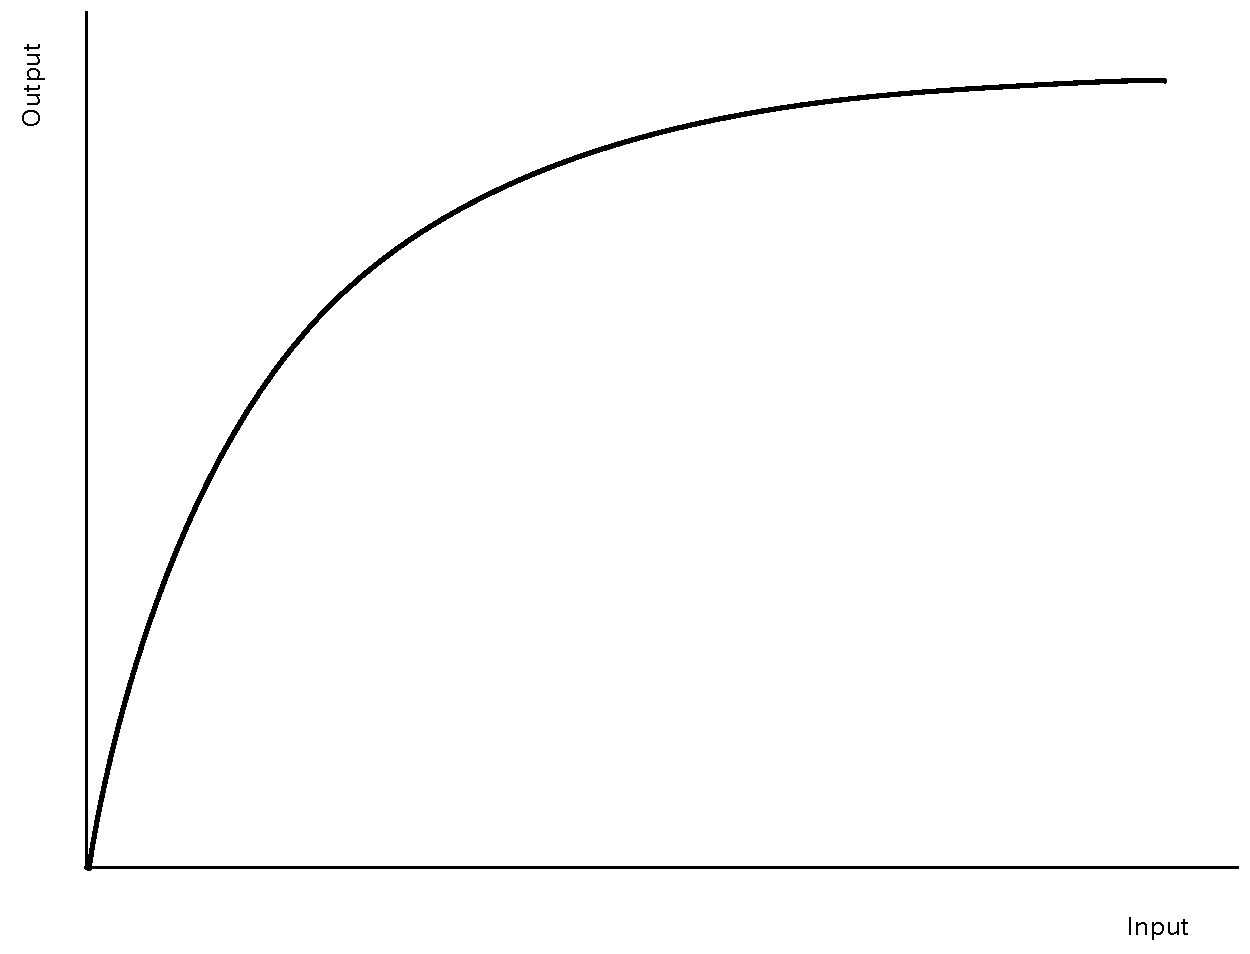
\includegraphics[scale=.40]{plot54.pdf}
		\caption{Bluth's Production Function}
		\label{mc2}
	\end{figure}

	Assume that the firm's only input is labor. Which of the following statements is TRUE?
	
	\begin{choices}
		\choice The production function exhibits economies of scale.
		\choice The production function exhibits increasing marginal product of labor.
		\choice The production function exhibits constant returns to scale.
		\CorrectChoice The production function exhibits diminishing marginal product of labor.
		\choice The production function exhibits diseconomies of scale.
	\end{choices}

\question If the prices of all goods and services produced in the economy rose while the quantity of all goods and services remained the same, which would rise?

\begin{choices}
	\CorrectChoice Nominal GPD, but not real GDP
	\choice Both nominal and real GDP
	\choice Real GDP, but not nominal GDP
	\choice Neither nominal nor real GDP
\end{choices}

\question Which of the following is \underline{not} an example of a barrier to entry?

\begin{choices}
	\choice A pharmaceutical company obtains a patent for a new medication to treat migraine headaches.
	\CorrectChoice A soybean farmer is the first in her country to use a new brand of fertilizer.
	\choice A taxi cab driver in New York City must obtain a license to legally provide transportation in the city.
	\choice Microsoft obtains a copyright for its Windows operating system.
\end{choices}
	

\uplevel{ Al's Burgers is a firm in a perfectly competitive market and faces the cost structure shown in Figure \ref{MC28}. Use this information for questions \ref{q3}-\ref{q4}.}
	
	\begin{figure}[H]
		\centering
		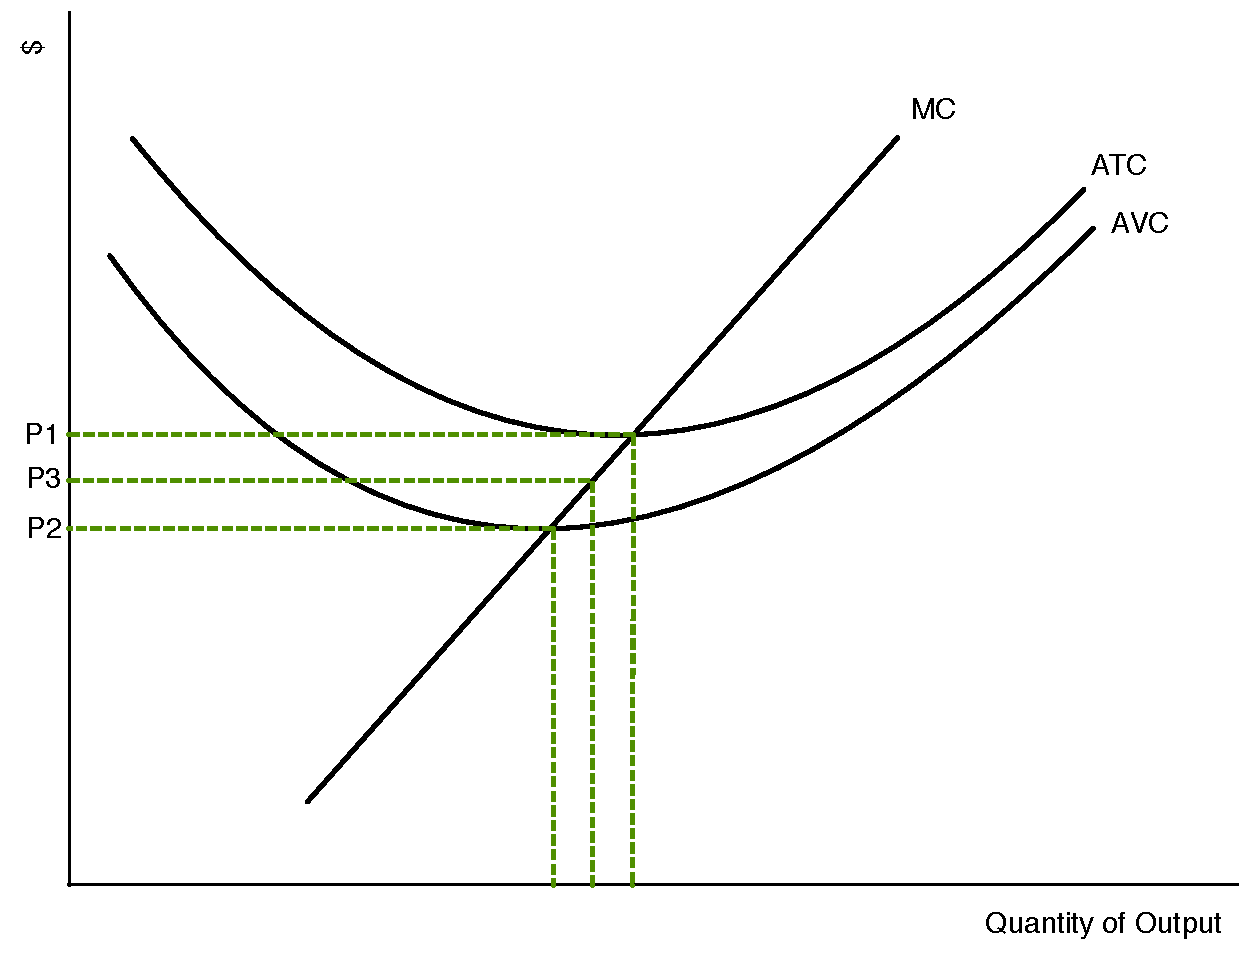
\includegraphics[scale=.40]{Exam1_MC27.pdf}
		\caption{Market for Fanta}
		\label{MC28}
	\end{figure}


\question \label{q3} Al's Burgers is currently making a profit $\Pi > 0$. Given this, the market price for burgers must be

	\begin{choices}
		\CorrectChoice greater than P1.
		\choice less than P2.
		\choice greater than P3 but less than P1.
		\choice greater than P2 but less than P3.
	\end{choices}



\question \label{q4} In the long-run, the price of burgers will be \blank and Al will produce a \blank\\ quantity burgers than they currently produce in the short-run. 

	\begin{choices}
	\CorrectChoice P1; smaller
	\choice less than P2; smaller
	\choice P2; smaller
	\choice more than P1; greater
	\choice greater than P2 but less than P1; greater
\end{choices}
	
\uplevel{A firm is currently in a market with the conditions outlined in Table \ref{SA3}. The firm has fixed costs of \$1,500 per day. Use this information to answer questions \ref{q5}-\ref{q6}.}

\begin{table}[H]
	\caption{Market Environment}
	\centering
	\begin{tabular}{c|c|c} 
		
		Quantity/day   & Total Revenue &  Marginal Cost \\
		\hline
		1 & \$600 &  \$1,000 \\
		2 & \$1,200 & \$400 \\
		3 & \$1,800 & \$500 \\
		4 & \$2,400 & \$600 \\
		5  & \$3,000 & \$800 \\
	\end{tabular}
	\label{SA3}
\end{table}

\newpage

\question \label{q5} If the firm produces 4 units of output, its total variable costs would be

\begin{choices}
	\choice \$2,000
	\choice \$500
	\choice \$167
	\choice \$1,900
	\CorrectChoice \$2,500
\end{choices}

\question \label{q6} In the short-run, the firm should \blank. Moreover, in the long-run the firm will \blank.

\begin{choices}
	\choice continue to operate in the short-run and produce 5 units of output in order to maximize profits; remain in the market
	\choice shutdown in the short-run and produce 0 units of output in order to maximize profits; remain in the market
	\choice continue to operate in the short-run and produce 4 units of output in order to maximize profits; exit the market
	\CorrectChoice shutdown in the short-run and produce 0 units of output in order to maximize profits; exit the market
	\choice continue to operate in the short-run and produce 4 units of output in order to maximize profits; remain in the market
\end{choices}


\question How many of the following statements regarding perfectly competitive markets are TRUE?

\begin{enumerate}[i.]
	\item Perfectly competitive markets are characterized by many buyers and sellers.
	\item In the long-run, firms in perfectly competitive markets operate at the quantity that minimizes average total costs.
	\item Firms in perfectly competitive markets are price takers and each individual firm faces a perfectly elastic demand curve.
	\item In the long-run, the process of entry and exit drives the profits of firms in perfectly competitive markets to zero.
\end{enumerate}

\begin{choices}
	\choice 3
	\choice 0
	\choice 2
	\CorrectChoice 4
	\choice 1
\end{choices}

	\question A family in Ireland purchases leather loafers that were produced by a shoemaker in Italy. As a result of this transaction, GDP in Ireland \blank and GDP in Italy \blank. 

\begin{choices}
	\choice increases; remains unchanged
	\CorrectChoice remains unchanged; increases
	\choice decreases; increases
	\choice increases; increases
	\choice increases; remains unchanged
\end{choices}

\question A monopolistically competitive firm will increase its production if at current production levels the 

\begin{choices}
	\choice marginal revenue is greater than the average total cost.
	\choice price is greater than the average total cost.
	\CorrectChoice marginal revenue is greater than the marginal cost.
	\choice price is greater than the marginal cost.
\end{choices}


	\question Consider the simultaneous move game between Key and Peele shown below, where the first number in each block is the payoff to Key and the second is the payoff to Peele.

\renewcommand{\gamestretch}{1.5}
\sgcolsep=25pt
\begin{figure}[H]\hspace*{\fill}%
	\begin{game}{2}{2}[Key][Peele] 
		&  Left & Right \\
		Top & 6, 4 & $x$, 2 \\
		Bottom & 1, 3 & 5, $y$ \\
	\end{game} 
	\hspace*{\fill}%
\end{figure}

If ``Top'' is the dominant strategy for Key and ``Left'' is the dominant strategy for Peele, then possible values of $x$ and $y$ are

\begin{choices}
	\choice $x=4$ and $y=2$.
	\choice $x=6$ and $y=4$.
	\CorrectChoice  $x=6$ and $y=2$.
	\choice $x=4$ and $y=4$.
\end{choices}

\question A bag of sugar is sold to Coca Cola for \$0.50, which uses this sugar to make Sprite that is sold to consumers for \$1.25. Another bag of of sugar is sold to Food Lion for \$1.25, where it is sold to consumers for \$2.75. Together, these transactions have what effect on GDP?

\begin{choices}
	\CorrectChoice Increase GDP by \$4.00
	\choice Increase GDP by \$1.75
	\choice Increase GDP by \$5.75
	\choice Increase GDP by \$3.00
\end{choices}

	\question Firms in monopolistically competitive markets are similar to monopolies in that they both \blank and are similar to firms in perfectly competitive markets in that they both \blank.

\begin{choices}
	\choice are price makers; produce at the efficient quantity
	\choice make positive profits in the short and long run; produce at the minimum of ATC in the long run
	\choice are in markets with barriers to entry; make zero economic profit in the long run
	\CorrectChoice charge a price above the marginal cost; can freely enter and exit the market
\end{choices}

\newpage

	\question If there is an increase in the price of blueberries that causes consumers to purchase fewer pounds of blueberries and more pounds of strawberries, but the ``typical basket'' used to calculate the CPI remains the same, the CPI will suffer from

\begin{choices}
	\CorrectChoice substitution bias.
	\choice bias due to the introduction of new goods.
	\choice bias due to unmeasured quality change.
	\choice base-year bias. 
\end{choices}

\uplevel{Use Figure \ref{MC10}, which represents the environment faced by a monopoly, for questions \ref{q9} -  \ref{q10}.} 

\begin{figure}[H]
	\centering
	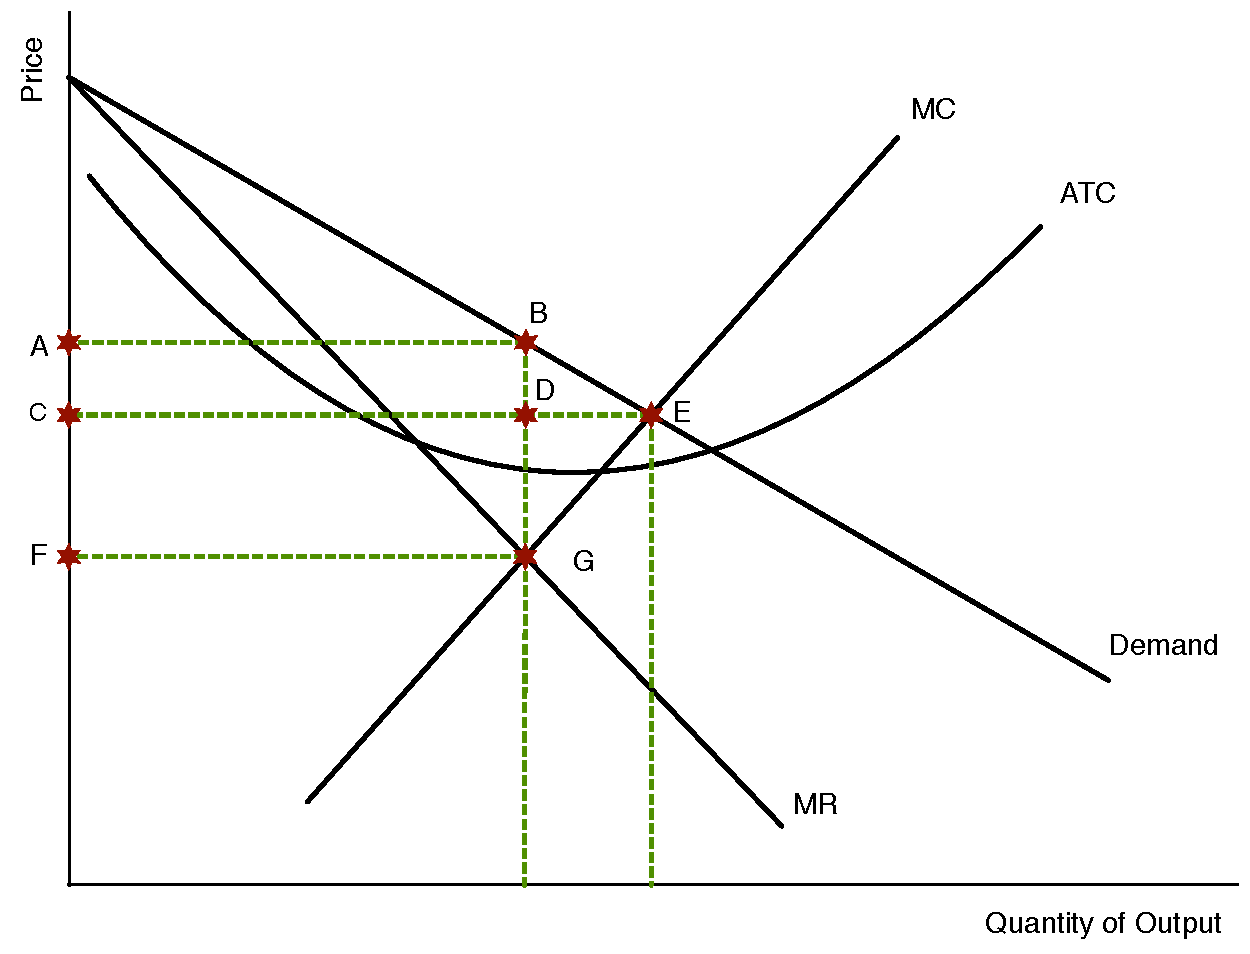
\includegraphics[scale=.4]{Exam2_MC10.pdf}
	\caption{Monopolist Environment}
	\label{MC10}
\end{figure}

\question \label{q9} Charging the price \blank maximizes the monopolist's profit, while total surplus would be maximized at price \blank.

\begin{choices}
	\choice C; A
	\CorrectChoice  A; C
	\choice F; C
	\choice A; F
\end{choices}


	\question \label{q10} Which of the following distances represents the mark-up over marginal cost at the profit maximizing quantity?

\begin{choices}
	\CorrectChoice Distance BG
	\choice Distance AC
	\choice Distance DE
	\choice Distance CF
\end{choices}

\newpage

	\question In 2014, an economy produced 100 apples that were sold for \$1.50 each and 125 oranges for \$2 each. The next year, the economy again produced 100 apples, but for \$1.25 each, and 140 oranges for \$2.25. Using 2014 as the base year, the GDP deflator in 2014 is \blank, while the GDP deflator in 2015 is \blank.

\begin{choices}
	\choice 98; 100
	\choice 102; 100
	\CorrectChoice 100; 102
	\choice 100; 98
\end{choices}
	

\uplevel{Table \ref{MC23} shows the prices and quantities produced of the only two goods in Uzbeki-beki-beki-Stan-Stan, grapes and olives, for the years 2000 and 2001. Assume 2000 is the base year. Use this information for questions \ref{q16}-\ref{q17}.}

\begin{table}[H]
	\caption{Grapes and Olives in UZN}
	\centering
	\begin{tabular}{c|c|c|c|c}
		Year & Grapes Produced & Price of Grapes & Olives Produced & Price of Olives \\
		\hline
		2000 & 20 & \$2.10 & 25 & \$4.10\\
		2001 & 20 & $x$ & 25 & $y$\\
	\end{tabular} 
	\label{MC23}
\end{table}

\question \label{q16} In 2001, the value of real GPD 

\begin{choices}
	 \choice is greater than real GDP in 2000.
	 \CorrectChoice is equal to real GDP in 2000.
	 \choice is less than real GDP in 2000.
	 \choice cannot be determined from this information.
\end{choices}


\question \label{q17} If nominal GDP was greater in 2000 than in 2001, how many of the following statements \textit{could} account for this?


\begin{enumerate}[(i)]
	\item $x = \$2.00$ and $y = \$4.10$
	\item $x = \$2.10$ and $y = \$4.40$
	\item  $x = \$2.20$ and $y = \$4.10$
	\item $x = \$2.10$ and $y = \$3.90$
\end{enumerate}

\begin{choices}
	\choice 0
	\choice 1
	\choice 3
	\CorrectChoice 2
	\choice 4
\end{choices}

\newpage

\question Which of the following regarding the relationship between average total costs and marginal costs is TRUE?

\begin{choices}
	\CorrectChoice If marginal costs are greater than average total costs, then it must be that average total costs are increasing.
	\choice If marginal costs are greater than average total costs, then it must be that marginal costs are decreasing.
	\choice If marginal costs are greater than average total costs, then it must be that average total costs are decreasing.
	\choice If marginal costs are less than average total costs, then it must be that marginal costs are decreasing.
\end{choices}


\question Consider the game matrix below.

\renewcommand{\gamestretch}{1.5}
\sgcolsep=25pt
\begin{figure}[H]\hspace*{\fill}%
	\begin{game}{3}{3}[Noah][Isabella] 
		&  Run & Walk & Crawl \\
		Run & 4, 1 & 4, 4 & 1, 2 \\
		Walk & 3, 4 & 1, 3 & 3, 2 \\
		Crawl & 2, 4 & 2, 3 & 4, 6 \\
	\end{game} 
	\hspace*{\fill}%
\end{figure}

How many Nash Equilibria does this game have?

\begin{choices}
	\choice 4 or more
	\choice 1
	\choice 0
	\choice 3
	\CorrectChoice 2
\end{choices}


\question How many of the following transactions would affect the consumption component of US GDP? Assume all of the transactions occur within the United States.

\begin{enumerate}[(i)]
	\item A family buys a new refrigerator.
	\item Jane purchases a used bookshelf from a friend.
	\item Jane's brother gets a haircut from his favorite barber.
	\item A newly-wed couple buys a newly constructed home.
\end{enumerate}

\begin{choices}
	\choice 1
	\choice 0
	\choice 3
	\CorrectChoice 2
	\choice 4
\end{choices}

\newpage	

	\question \textit{The New York Times} cost \$0.15 in 1970 and \$0.75 in 2000. If average wages in the US were \$3.23 per hour in 1970 and \$14.32 in 2000, then the purchasing power of workers in terms of $NYT$ newspapers 

\begin{choices}
	\choice was greater in 2000 than in 1970 because the average worker could purchase more newspapers in 2000 than in 1970.
	\choice was equal in 1970 and 2000 because the average worker could purchase the same number of newspapers in 2000 as in 1970.
	\CorrectChoice was greater in 1970 than in 2000 because the average worker could purchase more newspapers in 1970 than in 2000.
	\choice impossible to discern without more information.
\end{choices}

\question If a competitive firm were to double the quantity of output it sells, its

\begin{choices}
	\choice profits must increase.
	\choice marginal revenue must double.
	\CorrectChoice total revenue must double.
	\choice marginal cost must double.
\end{choices}


\question The price of large manufacturing machines declines. As a result, the GDP deflator \blank and the CPI \blank.

\begin{choices}
	\choice does not change; decreases
	\choice does not change; does not change
	\choice decreases; decreases
	\CorrectChoice decreases; does not change
\end{choices}

\question A firm is able to produce 165 units of output per day when 15 workers are hired. Additionally, the firm is able to produce 176 units of output per day when 16 workers are hired (holding other inputs fixed). The marginal product of the 16th worker is

\begin{choices}
	\choice 10 units.
	\choice 16 units.
	\CorrectChoice 11 units.
	\choice 176 units.
\end{choices}


\question A monopoly is an inefficient way to produce a product because 

\begin{choices}
	\choice monopolies produce too much of a good at too high of a price and thus will have inefficient transactions.
	\choice monopolies produce too little of a good at too low of a price thus will have unrealized gains from trade.
	\choice monopolies produce too much of a good at too low of a price thus will have inefficient transactions.
	\CorrectChoice monopolies produce too little of a good at too high of a price thus will have unrealized gains from trade.
\end{choices}

\newpage

\question Which of the following is true regarding the relationship between the \underline{output} produced by a monopoly, an oligopoly acting as a cooperative cartel, an oligopoly that is not cooperative, and a perfectly competitive (PC) firm?

\begin{choices}
	\choice monopoly < cooperative cartel < non-cooperative oligopoly < PC firm
	\CorrectChoice  monopoly = cooperative cartel < non-cooperative oligopoly < PC firm
	\choice  monopoly < cooperative cartel < non-cooperative oligopoly = PC firm
	\choice  monopoly = cooperative cartel = non-cooperative oligopoly < PC firm
\end{choices}

\question Which of the following is true regarding the relationship between the \underline{price} charged by a monopoly, an oligopoly acting as a cooperative cartel, an oligopoly that is not cooperative, and a perfectly competitive (PC) firm?

\begin{choices}
	\choice monopoly > cooperative cartel > non-cooperative oligopoly > PC firm
	\CorrectChoice  monopoly = cooperative cartel > non-cooperative oligopoly > PC firm
	\choice  monopoly > cooperative cartel > non-cooperative oligopoly = PC firm
	\choice  monopoly = cooperative cartel = non-cooperative oligopoly > PC firm
\end{choices}

\question Raymond left his job as a stock broker where he was earning \$70,000 a year to start a cookie business. Over the past year, Raymond sold 50,000 boxes of cookies at a price of \$4.00 per box. Also, over the course of the year, Raymond incurred labor costs of \$60,000 and paid \$20,000 for raw materials. Raymond's \underline{accounting} profit for the year was 

\begin{choices}
	\choice \$70,000.
	\CorrectChoice \$120,000.
	\choice \$50,000.
	\choice \$80,000.
\end{choices}


\question The goal of a firm in perfect competition is to maximize \blank, while the goal of a monopolist firm is to maximize \blank.

\begin{choices}
	\CorrectChoice profit; profit
	\choice profit; total surplus
	\choice total surplus; profit
	\choice total surplus; total surplus
\end{choices}

\question The expenditure approach to GDP adds together

\begin{choices}
	\CorrectChoice consumption spending, investment spending, government purchases, and net exports.
	\choice consumption spending, firm profits, government purchases, and net exports.
	\choice wages and salaries, rent, interest, and firm profits.
	\choice consumption, interest, government purchases, net exports, wages and salaries, rent, investment, and firm profits.
\end{choices}

\newpage

	\question Refer to Table \ref{tab2}. 

\begin{table}[H]
	\centering
	\caption{CPI and Minimum Wages}
	\label{tab2}
	\begin{tabular}{c|c|c}        
		
		Year & CPI & Minimum Wage \\
		\hline
		1983 & 100.0 & \$3.35 \\
		1984 & 103.9 & \$3.35 \\
		1985 & 107.6 & \$3.35 \\
		1986 & 109.6 & \$3.35 \\
		1987 & 113.6 & \$3.35 \\
		1988 & 118.3 & \$3.35 \\
		1989 & 124.0 & \$3.35 \\
		1990 & 130.7 & \$3.80 \\
	\end{tabular}
\end{table}

Given this information, which of the following statements are TRUE?

\begin{enumerate}[(i)]
	\item The standard of living for minimum-wage workers remained the same between 1985 and 1989 because the minimum wage remained the same.
	\item The standard of living for minimum-wage workers was higher in 1990 than in 1987 because a minimum wage worker's purchasing power was greater in 1990.
\end{enumerate}

\begin{choices}
	\CorrectChoice Neither i or ii
	\choice Only ii
	\choice Both i and ii 
	\choice Only i
\end{choices}	





\question If a firm faces multiple demand curves for their good (e.g., older individuals have a greater willingness to pay than younger individuals), but cannot perfectly price discriminate, imperfect price discrimination would

\begin{choices}
	\choice never be used because the firm's profits will be higher if they charge one price to all consumers.
	\CorrectChoice be used if possible because a firm's profits are always greater if they price discriminate.
	\choice never be used because price discrimination in any form is illegal.
	\item be used if possible because it will always increase total surplus in the market.
\end{choices}


\question The market for soybeans is perfectly competitive. It follows that the demand curve faced by any individual soybean producer for their output is 

\begin{choices}
	\CorrectChoice perfectly elastic.
	\choice unit elastic.
	\choice downward sloping.
	\choice perfectly inelastic.
\end{choices}




\uplevel{Table \ref{tab5} shows the prices and quantities consumed in some country. Assume that the typical basket of beef and pork was in determined 2014 and this is the base year. Use this information to answer questions \ref{q25}-\ref{q26}.}

\begin{table}[H]
	\centering
	\caption{Beef \& Pork}
	\label{tab5}
	\begin{tabular}{c|c|c|c|c}        
		
		Year & Price of Beef & Quantity of Beef & Price of Pork & Quantity of Pork \\
		\hline
		2014 & \$2.00 & 100  & \$1.00 & 100  \\
		2015 & \$2.50  & 90  & \$0.90 & 120  \\
		2016 & \$2.75  & 105  & \$1.00 & 130  \\
	\end{tabular}
\end{table}

\question \label{q25} What is the value of the CPI in 2015 (rounded to the nearest whole number)?

\begin{choices}
	\choice 125
	\choice 333
	\choice 300
	\CorrectChoice 113
	\choice 133
\end{choices}


\question \label{q26} Using the CPI, what was the inflation rate between 2014 and 2015 (rounded to the nearest whole number)?

\begin{choices}
	\choice $-10\%$
	\CorrectChoice 13\%
	\choice 10\%
	\choice $-13\%$
\end{choices}








\end{questions}
\end{document}